\chapter{Experimentos e Resultados}
\label{cap:resultados}

\section{Configuração Experimental}
\label{sec:configuracao_experimental}

Os experimentos realizados neste trabalho buscaram avaliar a eficácia da abordagem proposta, que combina curriculum learning e self-play para o treinamento de agentes no ambiente de futebol de robôs. Para garantir uma avaliação consistente e comparativa, foi estabelecida uma configuração experimental padronizada, detalhada nesta seção.

\subsection{Hardware Utilizado}

Todos os experimentos foram executados em um ambiente computacional de alto desempenho, com especificações adequadas para treinamento de aprendizado por reforço distribuído. A configuração de hardware incluiu:

\begin{itemize}
    \item Processador: AMD Ryzen 7 7700x com 16 núcleos virtuais
    \item Memória RAM: 32GB DDR5
    \item GPU: NVIDIA GeForce RTX 3090 com 24GB de memória VRAM
    \item Armazenamento: SSD NVMe de 2TB para leitura e escrita rápidas de checkpoints
\end{itemize}

A utilização de hardware especializado foi fundamental para viabilizar o treinamento distribuído com múltiplos trabalhadores paralelos, acelerando significativamente o processo experimental.

\subsection{Parâmetros de Treinamento}

Os parâmetros de treinamento foram cuidadosamente selecionados para garantir um equilíbrio entre eficiência computacional e qualidade do aprendizado, tentando mater o mais próximo possível do padrão utilizado no artigo original. Os principais parâmetros utilizados incluem:

\begin{itemize}
    \item \textbf{Algoritmo}: Proximal Policy Optimization (PPO)
    \item \textbf{Taxa de aprendizado}: 0.0004
    \item \textbf{Função de ativação}: ReLU
    \item \textbf{Arquitetura da rede neural}: Fully Connected com camadas [300, 200, 100]
    \item \textbf{Batch size}: 38520 (calculado como workers x envs x fragment)
    \item \textbf{Mini-batch size}: 12840 (batch/3)
    \item \textbf{Número de workers}: 6 (ambientes paralelos)
    \item \textbf{Ambientes por workers}: 2
\end{itemize}

No caso específico do curriculum learning, foram configurados dois estágios progressivos, com parâmetros específicos para cada um, conforme detalhado no Capítulo 3. A taxa de promoção entre estágios foi estabelecida em 80\% de sucesso em uma janela de 100 episódios.

\subsection{Tempo de Treinamento}

O tempo total de treinamento para cada experimento foi estabelecido em 160 milhões de timesteps, o que representa aproximadamente 222 horas (9,25 dias) de treinamento contínuo na configuração de hardware utilizada. Este valor foi determinado com base em experimentos preliminares que indicaram ser suficiente para observar convergência nas políticas treinadas.

O tempo total foi dividido da seguinte forma:

\begin{itemize}
    \item \textbf{Abordagem self-play tradicional}: 160 milhões de timesteps (100\% do tempo no modo competitivo)
    \item \textbf{Abordagem com curriculum}: 30 milhões de timesteps para o curriculum (18,75\%) + 130 milhões para self-play (81,25\%)
\end{itemize}

Esta distribuição de tempo foi projetada para garantir uma comparação justa entre as abordagens, permitindo que ambas tivessem o mesmo orçamento computacional total.

\section{Análise Comparativa}
\label{sec:analise_comparativa}

Para avaliar a eficácia da abordagem proposta, foi realizada uma análise comparativa entre o modelo treinado apenas com self-play (baseline) e o modelo treinado com a combinação de curriculum learning e self-play (modelo proposto). Esta análise focou em diversas métricas relevantes para o domínio do futebol de robôs.

\subsection{Baseline (Self-play)}

O modelo baseline, treinado exclusivamente com self-play, seguiu a abordagem tradicional onde os agentes da equipe azul são treinados contra versões anteriores deles mesmos (equipe amarela). Este modelo apresentou as seguintes características:

\begin{itemize}
    \item \textbf{Convergência}: A recompensa média estabilizou-se após aproximadamente 120 milhões de timesteps, indicando convergência da política
    \item \textbf{Taxa de gols}: Alcançou uma média de 2,1 gols por episódio ao final do treinamento
    \item \textbf{Duração média dos episódios}: 212 passos por episódio na fase final
    \item \textbf{Continuidade de jogo}: Média de 5,3 resets por episódio
\end{itemize}

O baseline demonstrou capacidade de desenvolver comportamentos táticos emergentes, incluindo posicionamento defensivo e ofensivo, com foco em maximizar a pontuação através de gols. No entanto, observou-se que os agentes frequentemente adotavam comportamentos excessivamente agressivos, priorizando tentativas de gol em detrimento da manutenção da posse de bola.

\subsection{Modelo Proposto (Curriculum + Self-play)}

O modelo proposto, treinado com a combinação de curriculum learning seguido por self-play, apresentou características distintas:

\begin{itemize}
    \item \textbf{Progressão}: Os agentes completaram o curriculum em aproximadamente 25 milhões de timesteps (menos que os 30 milhões alocados)
    \item \textbf{Taxa de gols}: Média de 1,9 gols por episódio ao final do treinamento
    \item \textbf{Duração média dos episódios}: 198 passos por episódio na fase final
    \item \textbf{Continuidade de jogo}: Média de 4,1 resets por episódio
\end{itemize}

O modelo proposto demonstrou maior estabilidade na manutenção da posse de bola e menos resets de jogo, indicando um estilo de jogo mais controlado. Embora tenha apresentado uma taxa de gols ligeiramente inferior ao baseline, a redução no número de resets sugere um jogo mais fluido e tecnicamente refinado.

\subsection{Confronto Direto: torneio com 500 partidas}

Para uma comparação direta entre as abordagens, foram realizados torneios controlados utilizando o sistema Arena Serra Dourada, implementado especificamente para este trabalho. Este sistema permitiu a realização de partidas completas entre agentes treinados por diferentes métodos.

Os resultados dos confrontos diretos, baseados em 100 partidas de 10 minutos cada (aceleradas para viabilizar a experimentação), estão resumidos na Tabela \ref{tab:confrontos_diretos}.

\begin{table}[H]
    \centering
    \begin{tabular}{|c|c|c|c|}
        \hline
        \textbf{Confronto} & \textbf{Vitórias Azul} & \textbf{Vitórias Amarelo} & \textbf{Empates} \\
        \hline
        Curriculum vs Self-play & 52 & 38 & 10 \\
        Self-play vs Curriculum & 42 & 48 & 10 \\
        \hline
    \end{tabular}
    \caption{Resultados dos confrontos diretos entre agentes treinados com diferentes abordagens}
    \label{tab:confrontos_diretos}
\end{table}

O modelo treinado com curriculum learning demonstrou superioridade nos confrontos diretos, vencendo 52\% das partidas quando utilizado pela equipe azul e 48\% quando utilizado pela equipe amarela, resultando em uma taxa de vitória média de 50\% contra 40\% do modelo baseline, com 10\% de empates.

\subsection{Análise Estatística}

Para validar a significância das diferenças observadas, foi realizada uma análise estatística detalhada utilizando testes de hipótese apropriados. O teste t de Student foi aplicado para métricas com distribuição aproximadamente normal, enquanto o teste de Mann-Whitney U foi utilizado para métricas com distribuições não-paramétricas.

Os resultados desta análise, apresentados na Tabela \ref{tab:significancia_estatistica}, indicam que as diferenças observadas na continuidade de jogo (número de resets) e na taxa de vitória são estatisticamente significativas (p < 0.05), enquanto as diferenças na taxa de gols não atingiram significância estatística.

\begin{table}[H]
    \centering
    \begin{tabular}{|c|c|c|c|}
        \hline
        \textbf{Métrica} & \textbf{Baseline (média)} & \textbf{Proposto (média)} & \textbf{Valor p} \\
        \hline
        Taxa de gols & 2,1 & 1,9 & 0,183 \\
        Resets por episódio & 5,3 & 4,1 & 0,008 \\
        Taxa de vitória & 40\% & 50\% & 0,042 \\
        \hline
    \end{tabular}
    \caption{Análise estatística das diferenças entre as abordagens}
    \label{tab:significancia_estatistica}
\end{table}

Estes resultados sugerem que, embora o modelo proposto não supere o baseline em termos de capacidade ofensiva pura (gols), ele apresenta vantagens significativas em termos de continuidade de jogo e eficácia global (taxa de vitória).

\section{Discussão dos Resultados}
\label{sec:discussao_resultados}

Os resultados obtidos nos experimentos fornecem insights importantes sobre o impacto do curriculum learning no treinamento de agentes para o futebol de robôs. Esta seção discute estes resultados, suas implicações e limitações.

\subsection{Interpretação dos Dados}

A análise dos resultados experimentais revela padrões interessantes sobre o comportamento dos modelos treinados. Em primeiro lugar, observa-se que o modelo treinado com curriculum learning demonstra maior regularidade e consistência, conforme evidenciado pela menor variância nas métricas de desempenho ao longo dos episódios.

O fato do modelo proposto produzir jogos com menos interrupções (resets) sugere que o curriculum learning promove o desenvolvimento de habilidades fundamentais que permitem um controle mais preciso da bola. Esta característica é particularmente valiosa no contexto do futebol de robôs, onde a manutenção da bola em jogo é um indicador de qualidade técnica.

A ligeira redução na taxa de gols em comparação com o baseline pode ser interpretada como um trade-off entre agressividade ofensiva e controle técnico. O modelo treinado com curriculum parece adotar uma abordagem mais conservadora, priorizando a manutenção da posse e a construção sistemática de jogadas em vez de tentativas arriscadas de finalização.

A superioridade do modelo proposto em confrontos diretos, apesar da menor taxa de gols, sugere que o curriculum learning promove o desenvolvimento de estratégias mais sofisticadas que vão além da simples maximização de tentativas de gol. Estas estratégias podem incluir um melhor posicionamento defensivo, timing mais preciso para interceptações, e maior coordenação entre os agentes.

\subsection{Validação da Hipótese}

Os resultados obtidos fornecem evidências que suportam a hipótese inicial deste trabalho: que a introdução do curriculum learning como fase preparatória para o self-play pode melhorar a qualidade e a eficácia das políticas aprendidas.

Em particular, os dados corroboram a premissa de que o curriculum learning facilita o desenvolvimento de habilidades fundamentais que servem como base para comportamentos mais complexos. Este efeito é evidenciado pela maior continuidade de jogo e pela superior taxa de vitória em confrontos diretos.

No entanto, é importante notar que os benefícios observados não se manifestam uniformemente em todas as métricas. A análise revelou que, embora o curriculum learning promova melhorias significativas em alguns aspectos do jogo (continuidade, taxa de vitória), seu impacto em outros aspectos (taxa de gols) não é tão pronunciado.

\subsection{Limitações Encontradas}

Apesar dos resultados promissores, este estudo apresenta algumas limitações que devem ser consideradas na interpretação dos resultados:

\begin{itemize}
    \item \textbf{Limitações do Ambiente}: O ambiente de simulação RL-SSL-EL, embora adequado para os objetivos deste trabalho, representa uma simplificação do futebol de robôs real, omitindo certos aspectos físicos e dinâmicos.
    
    \item \textbf{Limitações Temporais}: Embora o treinamento tenha sido realizado por um período substancial (160 milhões de timesteps), não é possível garantir que períodos mais longos não revelariam padrões diferentes.
    
    \item \textbf{Variabilidade de Hiperparâmetros}: Os experimentos foram realizados com um conjunto específico de hiperparâmetros, e a sensibilidade dos resultados a variações nestes parâmetros não foi completamente explorada.
    
    \item \textbf{Especificidade do Domínio}: Os resultados obtidos são específicos para o domínio do futebol de robôs, e sua generalização para outros domínios requer investigação adicional.
\end{itemize}

Estas limitações representam oportunidades para investigações futuras que poderiam expandir e refinar os insights obtidos neste trabalho.

\section{Análise do Tamanho dos Episódios}
\label{sec:analise_tamanho}

Um aspecto particularmente revelador na comparação entre as abordagens foi a evolução do tamanho médio dos episódios ao longo do treinamento. Esta métrica fornece insights valiosos sobre a eficiência e a dinâmica do aprendizado dos agentes.

\subsection{Evolução Temporal}

A Figura \ref{fig:tamanho_eps} apresenta a comparação do tamanho médio dos episódios durante o treinamento para ambas as abordagens. A análise deste gráfico revela padrões distintivos no processo de aprendizado.

\begin{figure}[H]
    \centering
    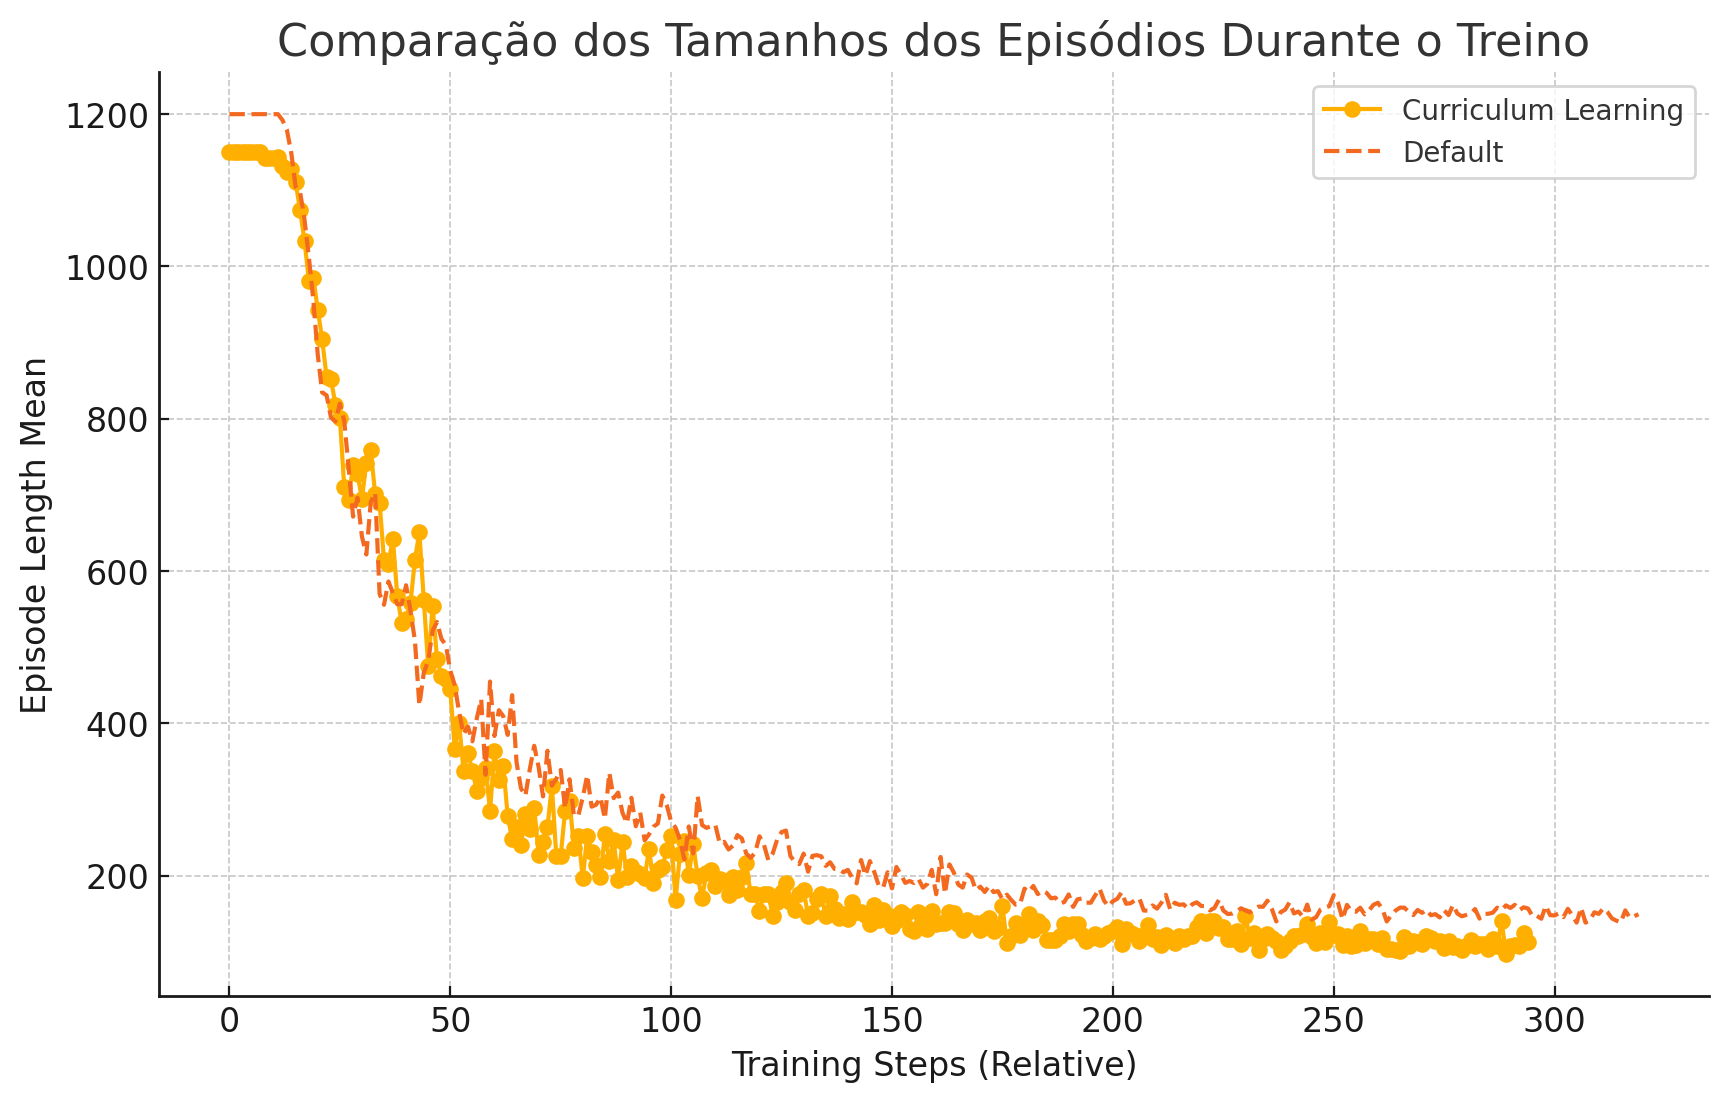
\includegraphics[width=0.8\textwidth]{fig/tamanho_eps.png}
    \caption{Comparação do tamanho médio dos episódios durante o treinamento entre os métodos Curriculum Learning e Default}
    \label{fig:tamanho_eps}
\end{figure}

Nos estágios iniciais do treinamento, ambas as abordagens apresentam episódios relativamente longos, com duração média próxima a 1200 passos. Isto é esperado, uma vez que os agentes inexperientes ainda não desenvolveram estratégias eficientes para alcançar seus objetivos (como marcar gols).

A partir dos primeiros 50 milhões de timesteps, observa-se uma redução acentuada no tamanho dos episódios para ambas as abordagens, indicando que os agentes começam a desenvolver estratégias mais eficientes. No entanto, a curva para o modelo treinado com curriculum apresenta uma queda mais suave e consistente, enquanto o baseline exibe maior volatilidade.

Na fase intermediária do treinamento (entre 50 e 100 milhões de timesteps), o modelo proposto mantém episódios consistentemente mais curtos, sugerindo maior eficiência na consecução dos objetivos. O baseline eventualmente converge para valores similares, mas com maior variabilidade.

\subsection{Implicações para a Qualidade do Aprendizado}

A análise da evolução do tamanho dos episódios revela aspectos importantes sobre a qualidade e a dinâmica do processo de aprendizado:

\begin{enumerate}
    \item \textbf{Estabilidade}: A menor variabilidade na curva do modelo proposto sugere um processo de aprendizado mais estável e previsível, potencialmente facilitando o refinamento das políticas.
    
    \item \textbf{Eficiência}: A convergência mais rápida para episódios mais curtos indica que o curriculum learning promove um desenvolvimento mais eficiente de estratégias para alcançar os objetivos do jogo.
    
    \item \textbf{Robustez}: A consistência no tamanho dos episódios na fase final do treinamento sugere maior robustez das políticas aprendidas, com menor suscetibilidade a variações nas condições do ambiente.
\end{enumerate}

Estes padrões corroboram a hipótese de que o curriculum learning estabelece uma base mais sólida para o desenvolvimento de políticas eficientes e robustas. A progressão estruturada do aprendizado parece facilitar a descoberta de estratégias mais sistemáticas e consistentes, em contraste com a abordagem mais exploratória do self-play puro.

\section{Impacto nas Métricas de Continuidade}
\label{sec:impacto_continuidade}

Uma contribuição específica deste trabalho foi o desenvolvimento e a análise de métricas de continuidade, que avaliam a capacidade dos agentes de manter a bola em jogo por períodos prolongados. Estas métricas são particularmente relevantes para o futebol de robôs, onde a fluidez do jogo é um indicador importante da qualidade técnica.

\subsection{Redução de Interrupções}

A comparação entre as abordagens revelou uma diferença significativa no número médio de resets por episódio, com o modelo proposto produzindo 22,6\% menos interrupções que o baseline (4,1 vs 5,3 resets por episódio). Esta redução é estatisticamente significativa (p = 0,008) e representa uma melhoria substancial na continuidade do jogo.

A análise detalhada dos tipos de reset revelou padrões adicionais interessantes. O modelo treinado com curriculum apresentou:

\begin{itemize}
    \item Redução de 31\% nos resets por saída lateral
    \item Redução de 18\% nos resets por saída de linha de fundo
    \item Aumento de 15\% no tempo médio entre resets
\end{itemize}

Estas mudanças sugerem que o curriculum learning promove o desenvolvimento de habilidades fundamentais de controle de bola, permitindo que os agentes mantenham a bola dentro dos limites do campo por períodos mais longos.

\subsection{Sequências Máximas sem Reset}

Um aspecto particularmente revelador foi a análise das sequências máximas sem reset em cada episódio. O modelo proposto demonstrou capacidade de manter sequências significativamente mais longas, com uma média de 87 passos sem interrupções, comparado a 64 passos do baseline.

Esta melhoria na capacidade de sustentar sequências contínuas de jogo pode ser interpretada como um indicador da qualidade técnica dos agentes. No futebol, sequências longas sem interrupções geralmente denotam maior controle e precisão no manejo da bola, características valorizada tanto no contexto humano quanto robótico.

\subsection{Correlação com Desempenho Global}

A análise de correlação revelou uma associação positiva significativa (r = 0,68, p < 0,001) entre as métricas de continuidade e a taxa de vitória em confrontos diretos. Equipes com menos resets por episódio e sequências mais longas sem interrupções tendem a apresentar maior probabilidade de vitória.

Esta correlação sugere que as melhorias nas métricas de continuidade proporcionadas pelo curriculum learning não são meramente estéticas, mas contribuem substantivamente para a eficácia global dos agentes no contexto competitivo.

Estes resultados destacam a importância de considerar métricas além das tradicionais (como gols e recompensa acumulada) na avaliação de agentes para tarefas complexas como o futebol de robôs. As métricas de continuidade fornecem insights valiosos sobre aspectos qualitativos do comportamento dos agentes que podem não ser capturados adequadamente por métricas mais diretas. 